\documentclass[12pt]{UoAthesis} 
\usepackage{booktabs} 
\usepackage{color}
\usepackage{graphics}
\thesistitle{Honours Dissertation}
\thesisauthor{Christopher James Thomson} 
\thesispdfkeywords{}
\thesisyear{2012}

\thesisabstract{This is a short summary of my work...} 

\acknowledgements{I would like to dedicate this work to..}

%%% The bibtex file where your references are stored 
\bibliography{main}
\begin{document}

%%% = = = DISSERTATION OVERVIEW = = =

% - INTRODUCTION - % 
% - - Molecular dynamics, what is it, why is it important to Chemical
%engineering.
% - - Leading into potentials, need for faster methods, more accurate methods.%
%Review of exisiting literature (Chapela, PRIME SPEADMD), what they've done,
%why its not as good as what you're going to do % 

% Outline of the thesis to come

% - Molecular Simulation 
% -- Newtonian mechanics F=MA, is it valid? 
% -- Forces from potentials (conservative forces) 
% Types of forces (gravitional (which is neglected)), pairwise forces 
% leading to intermolecular potentials.

% --- Give an example soft potential (LJ), Introduce a discrete -- 
% -potential,hard sphere is the prototypical discrete potential, -- 
% -but there are steppedpotentials too (Chapela). Talk about the -- 
% -advantages/disadvantages etc.

%%%% Lead out of the chapter with this 
% --- Introduce discrete potentials, say they need a special method of solution
%(EDMD).
% - Simulation Methods - % 
% - -Force Driven Simulators 
% - - - Introduction and general algorithm 
% - - -Integrators: Euler, Verlet, Velocity Verlet, Gear...lit review to find
%more recent ones
% - - - Optimization: neighbour lists, truncation of the potential 
%- - - Adv/Disadv? or just within other relevant topics 
% - - Event Driven Simulators % - - - Introduction and general algorithm 
% - - - Collision rules 
%Actually older than force based, although not as popular.
% - - - Optimization: neighbour lists, O(1) priority queue algorithms, time warp%algorithms
% - -Measuring System Properties % - - - Radial Distribution Function
 % - - -Temperature 
% - - - Pressure 
% - - - Coefficient of Diffusion 
% - Results - % 
%- 'Checking the simulators' - %
 % Direct comparision with Chapela
 % - Discussion- % 
% - Conclusions - % 
% - Recommendations for future work - % 
% - Appendices -% 
% - - Derivation of collision rule for stepped potentials %
%% = = = END OVERVIEW = = = %%%

\chapter{Introduction}

Process simulation packages have become an integral part of chemical
engineering design. Central to these simulation software packages is
the ability to calculate thermodynamic and transport properties of
fluids quickly and accurately. 

\chapter{Molecular Dynamics} 
\section{Introduction} 

The underlying assumption behind many molecular dynamics simulations
is that the particles move according to the laws of newtonian
mechanics. The effects fo quantum mechanics are usuallysmall unless
very light atoms (such as hydrogen or helium) are being simulated or
the particles are vibrating at very high rates \cite{Frenkel2002}

The fundamental identity of newtonian mechnanics is Newton's Second
Law of Motion \eqref{eq:Fma}. This equation allows the prediction of a
particle's trajectory provided that an initial position and velocity
is known; and the forces acting on that particle can be calculated for
any position or velocity.

\begin{equation}
  \vec{F} = m \vec{a}
  \label{eq:Fma} 
\end{equation}

If a force depends only on the position of a particle it is known as a
conservative force. Almost all forces considered in molecular dynamics
are of this type because atoms or molecules do not lose energy due to
friction or any other dissipative process.

Conservative forces can be further subdivided into forces that depend
either on absolute position such as gravity or forces can depend on
position relative to another particle (intermolecular forces). Gravity
is usually neglected in MD simulations as the mass of atoms and
molecules is very small.

%\begin{equation} 
%  \vec{F_i} = \sum_{j \not= i}^{}F_{i} 
%  \label{eq:pairwise}
%\end{equation}

While the forces caused by groups of particles should also be
considered, this would severly complicate the simulation, and hence is
often ignored.

In MD simulations the intermolecular forces are usually described
using potentials.

\subsection{Potentials} 
A potential is the function of potential energy with position, where
position is usually expressed as a set of orthogonal vectors such as
$x$, $y$ and $z$ in three dimensions. Conservative forces can be
calculated from their potential by equation
\ref{eq:forcePotential}. The gradient of the potential, denoted by
$\nabla$ is the partial differential of the potential in each
orthogonal direction.

\begin{equation} 
\vec{F}=-\nabla U 
\label{eq:forcePotential} 
\end{equation}

A very popular potential used in molecular dynamics simulations is the
Lennard-Jones potential \cite{Lennard-Jones1924} shown in figure
\ref{fig:ljPot} and equation \ref{eq:LJ} as it is simple yet gives
comparable results to experimental values.

\begin{equation} 
  U(r) = 4 \epsilon \left[ \left( \frac{\sigma}{r} \right)^{12}
    -\left( \frac{\sigma}{r} \right)^{6} \right] 
  \label{eq:LJ} 
\end{equation}
In equation \ref{eq:LJ}, $\epsilon$ is the depth of the energy well,
while $\sigma$ is the root of the Lennard-Jones potential which
corresponds to the change from attractive to repulsive forces (see
figure \ref{fig:ljForce}), this is taken to be the diameters of the
particles during the collision.

\begin{figure}[htp] 
  \begin{center}
    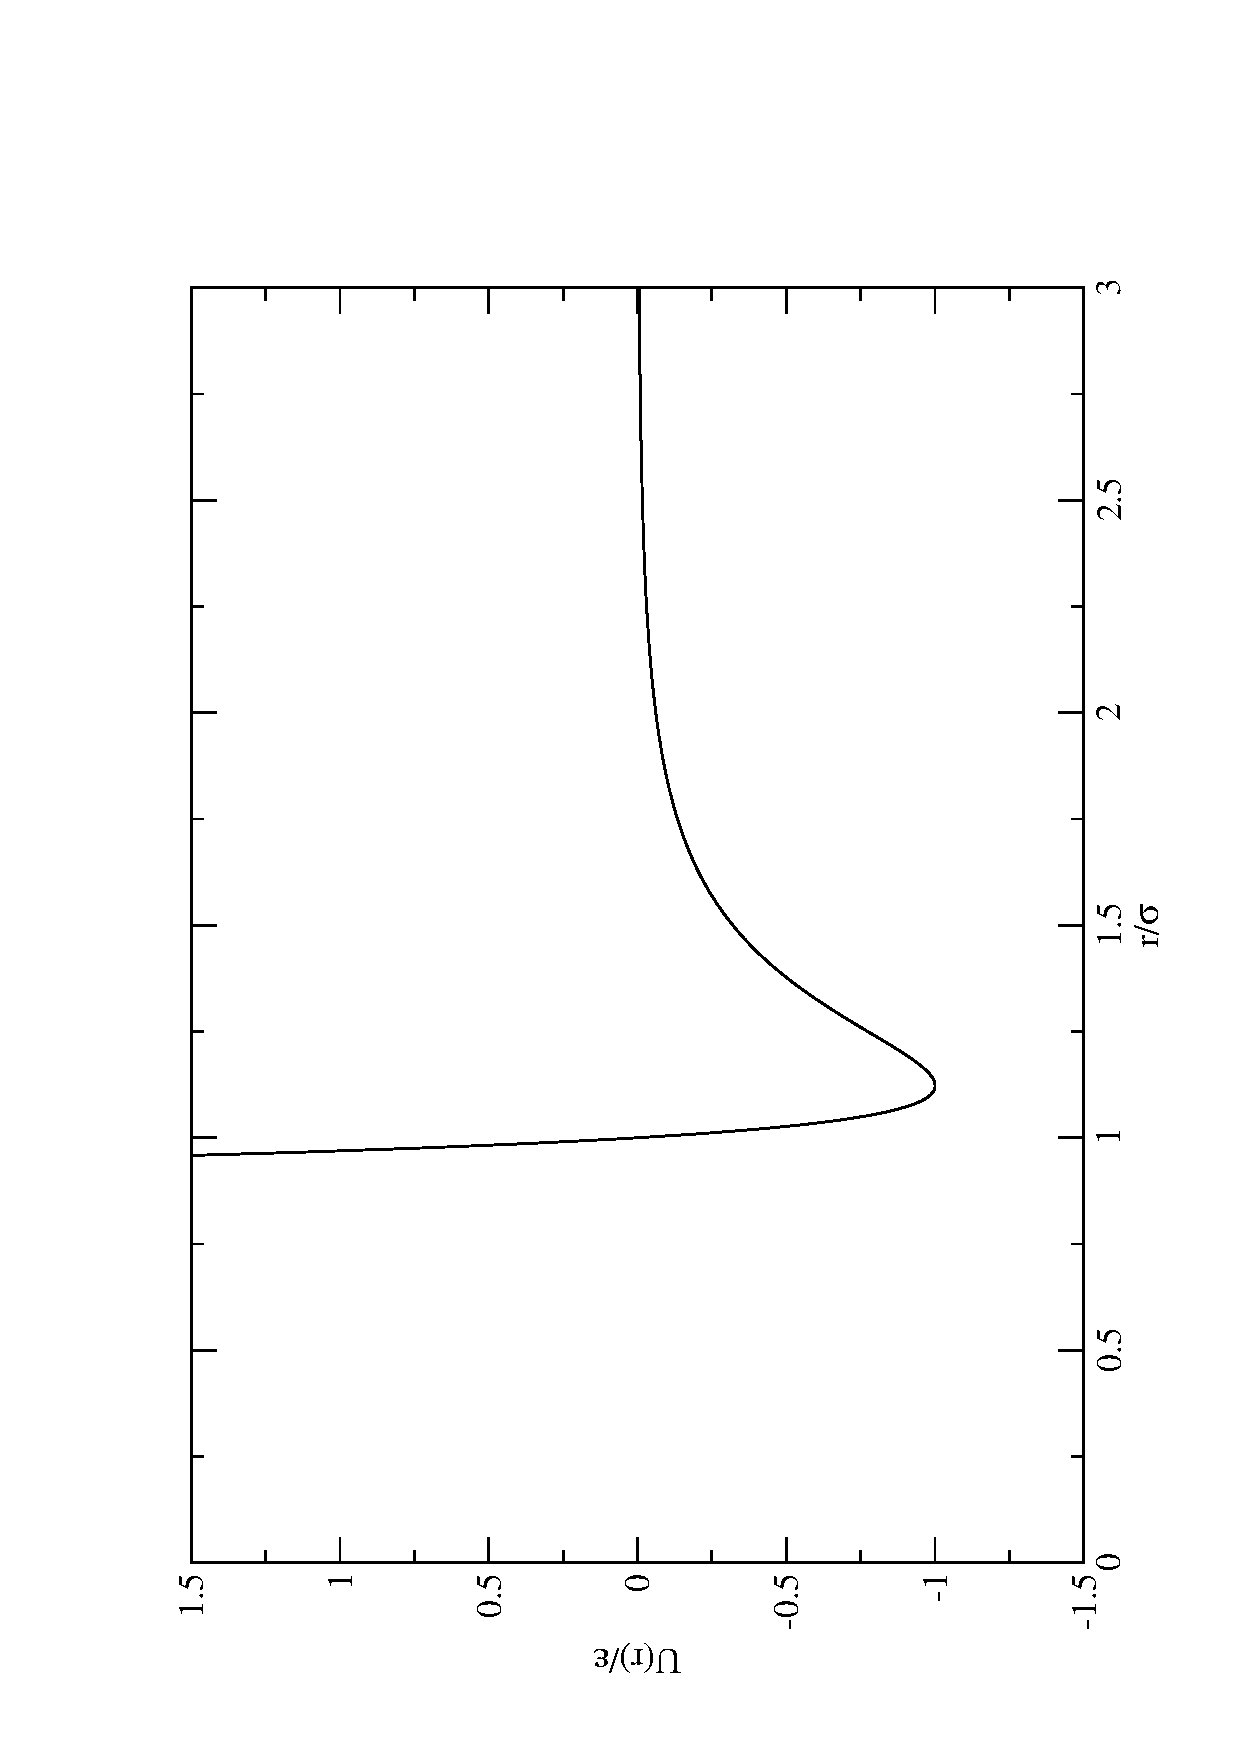
\includegraphics[clip,width=\textwidth]{figures/ljPlot} 
    \caption{\label{fig:ljPot} Plot of the Lennard-Jones potential} 
  \end{center}
\end{figure}

\begin{figure}[htp] 
  \begin{center}
    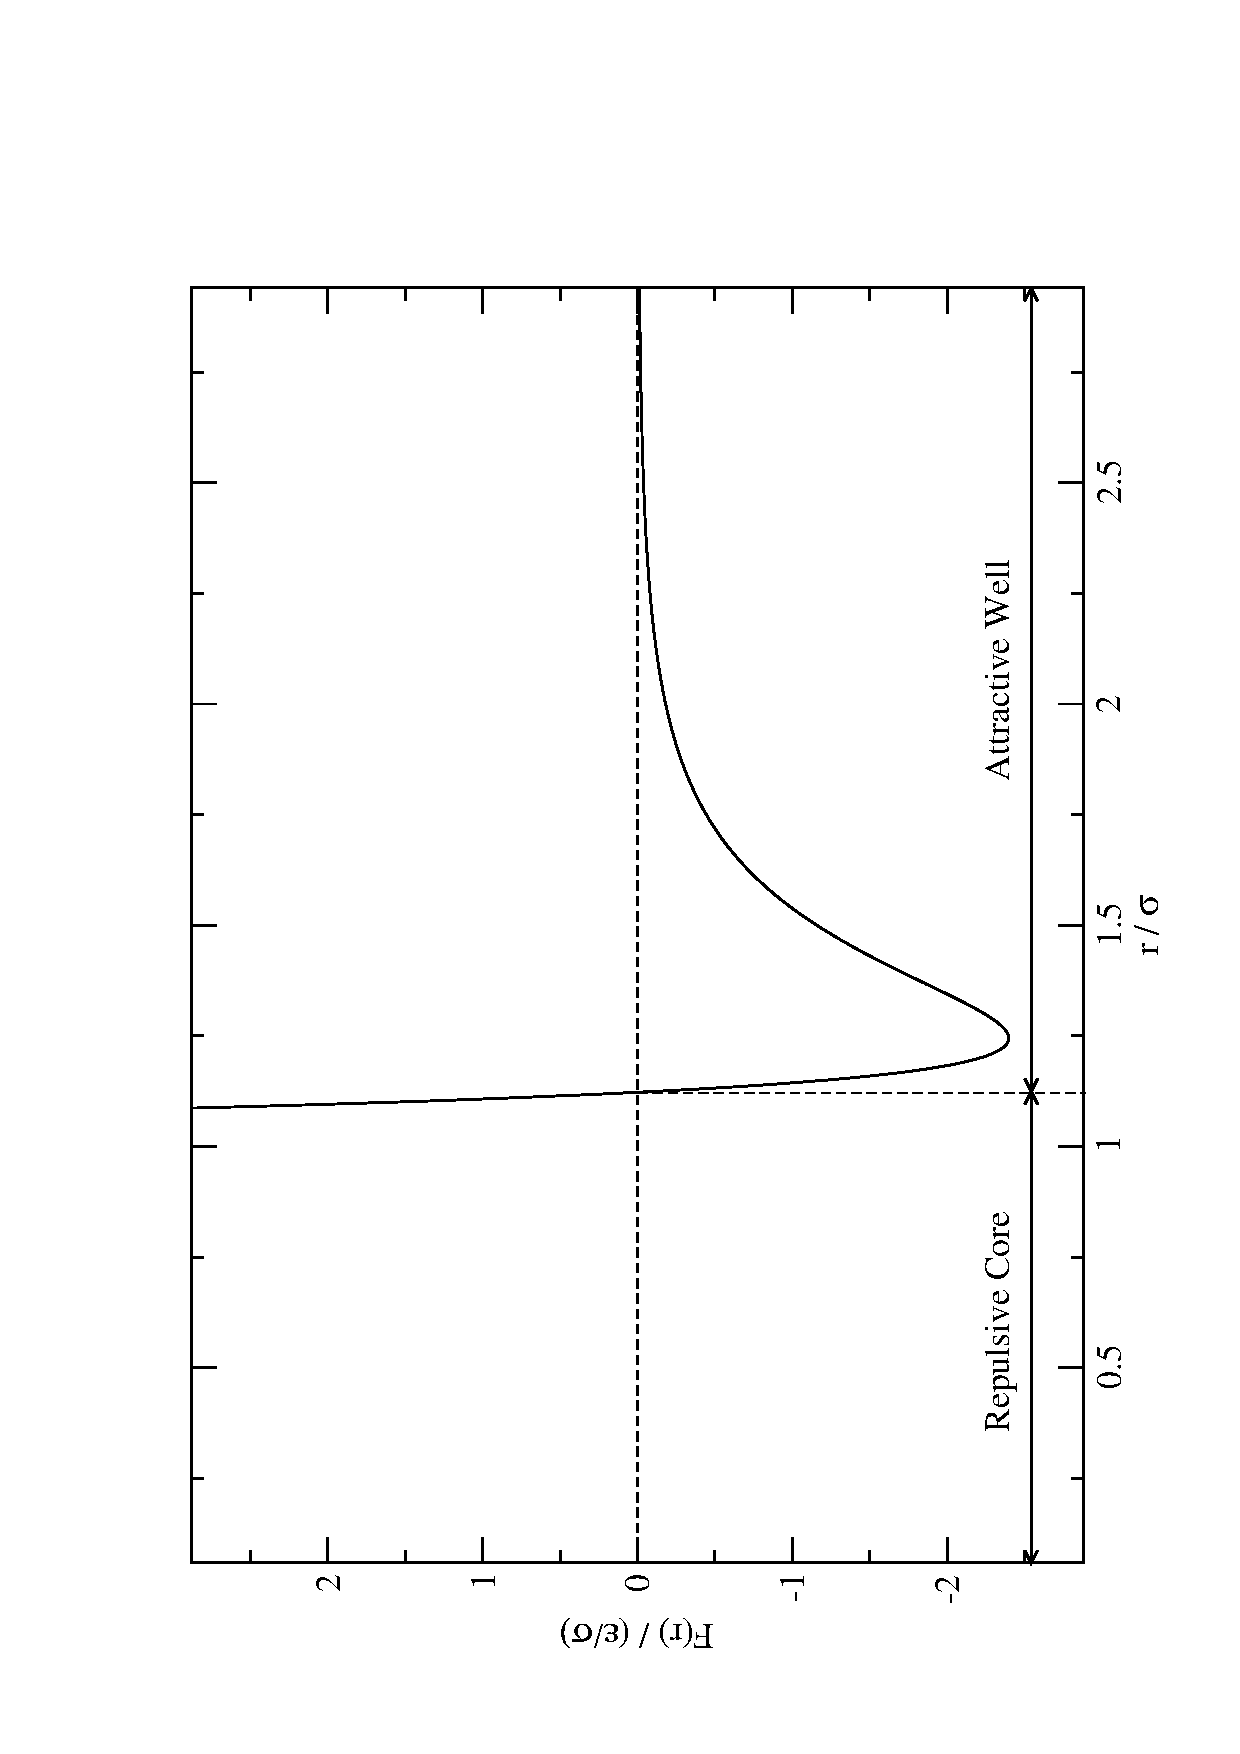
\includegraphics[clip,width=\textwidth]{figures/ljForce} 
    \caption{\label{fig:ljForce} Plot of the Lennard-Jones force between
      a pair of particles}
  \end{center}
\end{figure}
%[Insert plots of thelennard jones energy and force]% 
%[Insert massive potential from maginn possibly mention coulombs law, hertz's
%law?]
\newpage
\section{Force-Driven Simulators}
\subsection{Introduction} 
Force-driven (or time driven) simulators are the most popular method
of simulating particles due to their relative simplicity and ability
to handle soft potentials. Simulators of this kind were pioneered by
Rahman \cite{Rahman1964} who predicted physical properties of liquid
argon with reasonable accuracy.

The distinguishing feature between force-driven and event-driven
simulators is the way in which they move through time. During
force-based simulations particles' positions and velocities are
calculated every unit of time, $\Delta t$ using the forces acting on
the particles. These newly calculated values are then used to predict
the next set of particle positions. This is then repeated over the
desired simulation time.

\subsection{Integrators} 
Once the forces acting on a particle is known, that particle's
acceleration can be calculated using Newton's Second Law of Motion
(equation \ref{eq:Fmvdot}).

\begin{equation} 
  \vec{F} = m \frac{\partial^2 \vec{r}}{\partial t^2}
  \label{eq:Fmvdot} 
\end{equation}

However, since acceleration is the second time derivative of position
(velocity is the first time deriviative), calculating the particle's
future position results in solving a differential equation of order 2
or higher since force, andhence acceleration likely changes with
time. In order to accomplish this numerical integrators are used.

The majority of numerical integrators are based on Taylor Series
(equation \ref{eq:Taylor}).

\begin{equation} 
\vec{r}(t+\Delta t) = r(t) + 
\frac{\partial\vec{r}(t)}{\partial t}(\Delta t) + 
\frac{1}{2}\frac{\partial^2\vec{r}(t)}{\partial t^2}\Delta t^2 + 
\frac{1}{3!}\frac{\partial^3\vec{r}(t)}{\partial t^3}\Delta t^3 
+ \frac{1}{4!}\frac{\partial^4\vec{r}(t)}{\partial t^4}\Delta t^4 
+ ... \label{eq:Taylor} 
\end{equation}

The simplest integrator is Euler's Method which is just the Taylor
Series truncated after the acceleration term (equation
\ref{eq:Euler}).

\begin{equation} 
  \vec{r}(t+\Delta t) = r(t) + \vec{v}(\Delta t) +
  \frac{1}{2}\vec{a}\Delta t^2 + \mathcal{O}(\Delta t^3) 
  \label{eq:Euler}
\end{equation}

However this method suffers from large errors and is unstable
\cite{Haile1997} and is therefore rarely used. The Verlet Integrator
\cite{Verlet1967} improves upon Euler's method by combining the
forward timestep with a reverse timestep \eqref{eq:Verletpos}. This
method is actually fourth order as the third (and first) derivative is
cancelled out during its derivation. The Verlet integrator does not
include an equation to calculate the future velocity so the central
difference used by Verlet is often used \eqref{eq:VerletVel}.

\begin{subequations} 
  \begin{align} 
    \vec{r}(t + \Delta t) &= 2\vec{r}(t) - \vec{r}(t - \Delta t) 
    + \vec{a}(t)\Delta t^2 + \mathcal{O}(\Delta t^4)
    \label{eq:Verletpos} \\
    \vec{v}(t+\Delta t) &= \frac{\vec{r}(t+\Delta t) -
      \vec{r}(t-\Delta t)}{2\Delta t} 
    \label{eq:VerletVel} 
  \end{align}
\end{subequations}

Integrators suffer from couple key failings that cause a systematic
gain of energy known as ``energy drift''. Firstly, integrators are
based on infinite Taylor series which cannot be fully implemented,
therefore they have to be truncated after a certain number of terms,
this introduces an error. Secondly, integrators struggle to predict
values of forces that have discontinuities in them, such as hard
spheres which only have forces on contact but not before, or
discontinuities introduced by truncating potentials to improve
simulator speed.  There are a couple of types of integrators that try
and reduce these problems.

Sympletic integrators have the useful property in that they, on
average, conserve energy \cite{Hairer2003}. The most common symplectic
integrator used in MD is the Velocity Verlet Integrator
\cite{Swope1982} shown in \eqref{eq:VVerlet}.

\begin{subequations}
\label{eq:VVerlet}
\begin{align}
 \vec{r}(t + \Delta t) &= \vec{r}(t) + \vec{v}(t) \Delta t 
 + \frac{1}{2}\vec{a}(t) \Delta t^2 + \mathcal{O}(\Delta t^4)
 \label{eq:VVerletpos} \\
 \vec{v}(t+\Delta t) &= \vec{v}(t) + \frac{\vec{a}(t) 
   + \vec{a}(t+\Delta t)}{2}\Delta t
 \label{eq:VVerletVel}
\end{align}
\end{subequations}

The popularity of the Velocity Verlet is due to its computational
simplicity andits accuracy and stability at relatively long
timesteps. It can even be expanded\cite{Khakimov2002} to maintain its
accuracy and stability at very long timesteps at a small extra
computational cost. However the Velocity Verlet cannot be used in
systems that do not conserve energy, ie systems with dissipative
forces.

Another popular method of improving the traditional integrator is
predictor-corrector integrators. These use a truncated Taylor series
to calculated a predicted value for the future position and higher
order time derivatives. The force is then calculated at this
predicited position, then the difference between the predicted
acceleration and the corrected acceleration calculated from the force
is used to correct the position and time derivatives.

The most popular predictor-corrector integrator is that of Gear
\cite{Gear1971},using his 5th order algorithm. The predicted value for
the $i^{th}$ time derivative is shown in \eqref{eq:GearPredictor}, and
defining $\Delta \vec{a} = \vec{a}\,^{C} - \vec{a}\,^{P}$, the
corrected time derivatives can be calculated using
\eqref{eq:GearCorrector} with coefficients from \eqref{eq:GearCoeff}.

\begin{equation} 
  \frac{\partial^{i}}{\partial t^{i}} \vec{r}\:^{P}(t+\Delta t)
  =\sum^{n}_{k=i} \frac{1}{k!}\frac{\partial^{i} }{\partial t^{i}}
  \vec{r}(t) \Delta t^{k} 
  \label{eq:GearPredictor} 
\end{equation}

\begin{equation} 
  \frac{\partial^{i}}{\partial t^{i}} \vec{r}\:^{C}(t+\Delta t)
  =\frac{\partial^{i} }{\partial t^{i}} \vec{r}\:^{P}(t+\Delta t)
  +\frac{c_i}{\Delta t^i} \left(\frac{\Delta t^2}{2}\Delta \vec{a}\right)
  \label{eq:GearCorrector} \end{equation} \begin{equation} c_0 =
  \frac{3}{16},\;\;c_1 = \frac{251}{360},\;\; c_2 = 1,\;\; c_3 =
  \frac{11}{18},\;\; c_4 =
  \frac{1}{6},\;\; c_5 = \frac{1}{60} \label{eq:GearCoeff} 
\end{equation}

The Gear's algorithm, while more accurate at short timesteps than Verlet's
integrator \cite{Haile1997}, suffers at long timesteps and is computationally
more expensive.
\newpage
\section{Event-Driven Simulators} 
\subsection{Introduction} 
Though force-driven simulators are more popular the first MD
simulation was done using an event-driven simulator by Alder and
Wainwright \cite{Alder1959}. The difference between force and event
driven simulations lies in how the simulators move through time.
While force driven simulators move forward in uniform blocks, event
driven simulators jump between successive collisions.  These
collisions are taken to be instantaneous and only one can occur at any
particular time.

\subsection{Collision Time Prediction}
An event-driven simulator first must calculate the collision times
between every pair of particles (provided the particles do collide),
in order to select the earliest collision.  For hard sphere
simulations there are two conditions that must be satisfied in order
for a collision to occur.  Firstly, the particles must be moving
towards each other and secondly, the particles must pass close enough
to each other to collide.  These conditions can be expressed
mathematically in equations \eqref{eq:collConditions1} and
\eqref{eq:collConditions2} respectively \cite{Haile1997}.

\begin{subequations}
  \begin{align}
    \mathbf{v}_{ij}\cdot\mathbf{r}_{ij} < 0 \label{eq:collConditions1}\\
    (\mathbf{v}_{ij}\cdot\mathbf{r}_{ij})^2 
    - v_{ij}^2(r_{ij}^2 - \sigma^2) \geq 0 \label{eq:collConditions2}
  \end{align}
\end{subequations}

The time to collision can then be calculated using the quadratic in
equation \eqref{eq:collEnterTime}.  While there are two solutions,
only the earliest collision (the negative root) needs to be
considered.  The second root gives the time when the particles leave
after passing through each other which, for hard sphere, cannot
happen.

\begin{equation}
\Delta t = \frac{(-\mathbf{v}_{ij}\cdot\mathbf{r}_{ij}) \pm 
  \sqrt{(\mathbf{v}_{ij}\cdot\mathbf{r}_{ij})^2 - v_{ij}^2(r_{ij}^2 - \sigma^2)}}
       {v_{ij}^2} \label{eq:collEnterTime}
\end{equation}

Since $\mathbf{v}_{ij}\cdot\mathbf{r}_{ij}$ must be negative for the
collision, there is the possibility of catastrophic cancellation
\cite{Goldberg1991}, if $(\mathbf{v}_{ij}\cdot\mathbf{r}_{ij})^2 \gg
v_{ij}^2(r_{ij}^2 - \sigma^2)$. Therefore it is advisable to use the
positive root from the alternate form of the quadratic equation given
in equation \eqref{eq:collEnterTimeAlt} \cite{Poschel2005}.

\begin{equation}
\Delta t = \frac{r_{ij}^2 - \sigma^2}{(-\mathbf{v}_{ij}\cdot\mathbf{r}_{ij})
  \mp \sqrt{(\mathbf{v}_{ij}\cdot\mathbf{r}_{ij})^2 
    - v_{ij}^2(r_{ij}^2 - \sigma^2)}}
\label{eq:collEnterTimeAlt}
\end{equation}

When considering stepped potentials many of the same principles apply,
except there are now two possible ``collisions''. The first, when two
particles enter a step is treated identically to hard spheres. The
other event, when the particles leave the step, is calculated using
the second, later root of the quadratic.  In order to prevent loss of
numerical precision, the leaving time should be calculated using
equation \eqref{eq:collExitTime}.

\begin{equation}
  \label{eq:collExitTime}
\Delta t = 
\begin{cases}
  \frac{r_{ij}^2 - \sigma^2}{(-\mathbf{v}_{ij}\cdot\mathbf{r}_{ij})
    - \sqrt{(\mathbf{v}_{ij}\cdot\mathbf{r}_{ij})^2 
      - v_{ij}^2(r_{ij}^2 - \sigma^2)}}, & \text{if }
  \mathbf{v}_{ij}\cdot\mathbf{r}_{ij} > 0 \\
\\

\frac{(-\mathbf{v}_{ij}\cdot\mathbf{r}_{ij}) +
  \sqrt{(\mathbf{v}_{ij}\cdot\mathbf{r}_{ij})^2 - v_{ij}^2(r_{ij}^2 - \sigma^2)}}
     {v_{ij}^2} , & \text{if }
     \mathbf{v}_{ij}\cdot\mathbf{r}_{ij} < 0 
\end{cases}
\end{equation}

\subsection{Collision Dynamics}
Once the time of the next collision is known, the particles can be moved
to their new locations.  Generally there is no external force applied
to the particles in event-driven molecular dynamics, therefore the
particles move in straight lines.  Hence the particles' new positions
can be calculated using equation \eqref{eq:edNewPos}.

\begin{equation}
  \mathbf{r}(t+\Delta t) = \mathbf{r}(t) + \mathbf{v}(t)\Delta t 
  \label{eq:edNewPos}
\end{equation}

The post-collision velocities of the colliding particles must now be
calculated.  The simplest collision between two particles is an
elastic bounce, where the velocities and just exchanged along the
separation vector between the two particles.  The change in velocity
during the collision for particles $i$ and $j$ is shown in equation
\eqref{eq:postVBounce}.

\begin{subequations}
  \label{eq:postVBounce}
  \begin{align}
    \Delta\mathbf{v}_i &= -(\mathbf{v}_{ij}\cdot\mathbf{\hat{r}}_{ij})\mathbf{\hat{r}}_{ij} \\
    \Delta\mathbf{v}_j &= (\mathbf{v}_{ij}\cdot\mathbf{\hat{r}}_{ij})\mathbf{\hat{r}}_{ij}
  \end{align}
\end{subequations}

For stepped potential system, the collision dynamics are more complex.
When two particles collide they must pay an energy ``cost'' to proceed
through the step.  This energy cost $\Delta U$ is the difference in
the energy of the current step and the step the particles are going
into, and is shown in equation \eqref{eq:energyCost}.

\begin{equation}
  \label{eq:energyCost}
  \Delta U = U_{\text{next step}} - U_{\text{current step}}
\end{equation}

If the kinect energy of the particles is insufficient, the pair bounce
off the step and the post-collision velocities are calculated using
equation \eqref{eq:postVBounce}. However, if the particles can pay
this cost i.e.\ the inequality \eqref{eq:kineticCost} is true, then the
particles can enter the step.

\begin{equation}
\label{eq:kineticCost}
  \frac{1}{4}m(\mathbf{v}_{ij}\cdot\mathbf{\hat{r}}_{ij})^2 > \Delta U
\end{equation}

The change in the velocities of particles $i$ and $j$ after going
through a step are shown in equation \eqref{eq:postVCapture} where $A$
is given in equation \eqref{eq:changeMomentum}, the derivation of
these equations is given in Appendix ???.  If the particles are
entering a step, the positive root of $A$ is used, whereas if the
particles are leaving a step it is the negative root that should be
used.

\begin{subequations}
  \label{eq:postVCapture}
  \begin{align}
    \Delta\mathbf{v}_i &= \frac{A}{m} \mathbf{\hat{r}}_{ij} \\
    \Delta\mathbf{v}_j &= -\frac{A}{m}\mathbf{\hat{r}}_{ij}
  \end{align}
\end{subequations}

\begin{equation}
  \label{eq:changeMomentum}
  A = -\frac{m}{2}\left((\mathbf{v}_{ij}\cdot\mathbf{\hat{r}}_{ij}) \pm
  \sqrt{(\mathbf{v}_{ij}\cdot\mathbf{\hat{r}}_{ij})^2 - \frac{4}{m}\Delta U}\right)
\end{equation}
\newpage
\chapter{Methodology} 
\section{Introduction} 

The two simulators described in this chapter were coded in C++ using
the C++ Standard Library with the Boost [cite] library to handle
random number generation.

\section{Force-driven Simulator} 
Force driven simuators are currently the
dominant MD paradigm therefore it was decided that the results from
the stepped potentials would be compared to the equivalent results
obtained from a force-driven simulator. In order to acquire these
results a force-driven simulator was written.

The algorithm for the force driven simulator is as follows. 
\begin{flushleft}
  \begin{enumerate} 
  \item Initialisation 
  \item Calculate particles' future positions 
  \item Calculate the forces acting on the particles 
  \item Calculate the future velocities of particles 
  \item Run thermostat (if enabled) 
  \item Measure properties 
  \item Repeat steps 2-6 for the desired number of iterations
  \end{enumerate} 
\end{flushleft}

\subsection{Initialisation} The particles are initialised in a Face Centered
Cubic (FCC) \nomenclature[A]{FCC}{Face Centered Cubic} structure. The
use of the FCC lattice is common when simulating Lennard-Jones
potentials as the first force-driven simulation \cite{Rahman1964} was
carried out using liquid Argon which crystalises to a FCC lattice.

Particle velocities are assigned randomly from a Gaussian distribution
with a mean, $\mu = 0$, and a standard deviation, $\sigma =
\sqrt{T^{*}}$, where $T^{*}$ is the desired reduced temperature. The
velocities are then rescaled to ensure there net shift in linear
momentum in any direction by applying \eqref{eq:zeroLinearP} in each
orthongonal direction.

\begin{equation} 
  v_{i}^{new} = v_{i}^{old} - \frac{1}{N}
  \sum^{N}_{i}v_{i}^{old}
  \label{eq:zeroLinearP} 
\end{equation}

\subsection{Running Simulation} 
The
\chapter{Results} 
\section{Benchmarking} 
\subsection{Introduction} 
After a MD simulator has been created it is necessary to compare its
results with those generated by others, to verify that the simulator
works correctly.

\subsection{Event-Driven Simulator}
 The event-driven simulator was first tested running a hard sphere
 simulation before testing the more complex stepped potentials. A
 single 'step' with a energy requirement sufficiently large such that
 no particle could enter it. The simulation was run once at a range of
 densities using 864 particles at a reduced temperature of $T^*=1$ for
 5 million collisions, the results were compared with those of Lue
 \cite{Lue2005} in table \ref{tab:benchhard}. The agreement between
 results is good and lies within statistical uncertainty. The largest
 discrepancies are in the values for the coefficient of diffusion at
 low densities which is probably due to Lue's values were obtained
 after 10 million collisions.

\begin{table} \caption{Comparison of results obtained by the event-driven
simulator with literature values. $t_{avg}$ is the average time
between collisions, $\langle\mathbf{\hat{r}} \cdot \Delta \mathbf{v}
\rangle_{coll}$ is the average momentum transfer per collision, and D
is the coefficient of
diffusion.} \label{tab:benchhard} \begin{center} \begin{tabular}{l c c
        c c c c} \toprule $\rho$ & \multicolumn{2}{c}{$t_{avg}$} &
      \multicolumn{2}{c}{$\langle\mathbf{\hat{r}} \cdot \Delta
        \mathbf{v} \rangle_{coll}$} & \multicolumn{2}{c}{D}
      \\ \cmidrule(rl{0.75em}){2-3} \cmidrule(rl{0.75em}){4-5}
      \cmidrule(rl{0.75em}){6-7} & Simulator & Lue & Simulator & Lue &
      Simulator & Lue\\ \midrule 0.3 & 0.3052 & 0.3052 & 1.775 & 1.772
      & 0.53 & 0.55 \\ 0.4 & 0.1944 & 0.1942 & 1.776 & 1.773 & 0.341 &
      0.359 \\ 0.5 & 0.13024 & 0.13031 & 1.774 & 1.7724 & 0.247 &
      0.247 \\ 0.6 & 0.08966 & 0.08968 & 1.771 & 1.7721 & 0.169 &
      0.173 \\ 0.7 & 0.0625 & 0.0625 & 1.773 & 1.776 & 0.114 & 0.113
      \\ 0.8 & 0.04365 & 0.0436 & 1.772 & 1.772 & 0.064 & 0.065 \\ 0.9
      & 0.03029 & 0.03024 & 1.773 & 1.772 & 0.033 & 0.0327
      \\ \bottomrule
\end{tabular} \end{center} \end{table}

The simulator was then benchmarked using a step potential. The results
were compared with Chapela et al \cite{Chapela1989} using their 'Case
6' steps. The simulation was run for 1.5 million collisions using 864
particles. Each simulation was run ten times and the mean values and
standard deviations are given in table
\ref{tab:benchsoft} 

\begin{table} 
  \caption{Comparison of results
    obtained by the event-driven simulator with literature values
    using stepped potentials. Numbers in parenthesis indicate the
    uncertainty in the final digit.
\label{tab:benchsoft}} 
  \begin{center} 
    \begin{tabular}{l c c c c c c} 
      \toprule
      $\rho$ & \multicolumn{2}{c}{$\langle T\rangle$} &
      \multicolumn{2}{c}{$\langle U \rangle$} &
      \multicolumn{2}{c}{$\langle P \rangle$}
      \\ \cmidrule(rl{0.75em}){2-3} \cmidrule(rl{0.75em}){4-5}
      \cmidrule(rl{0.75em}){6-7}& Simulator & Chapela et al &
      Simulator & Chapela et al & Simulator & Chapela etal\\ 
      \midrule
      0.85 & 0.719(3) & 0.72 & -6.04(7) & -5.80 & -0.5(4) & 0.54
      \\ 0.85& 1.339(8) & 1.34 & -5.130(9) & -5.14 & 4.08(4) & 4.08
      \\ 0.85 & 2.35(1) & 2.35 & -4.24(2) & -4.20 & 8.78(9) & 8.86
      \\ 0.85 & 3.37(2) & 3.37 & -3.48(2) & -3.49 & 12.90(9) & 13.00
      \\ 0.85 & 4.59(1) & 4.60 & -2.67(1) & -2.68 & 17.31(8) & 13.43
      \\ 0.75 & 0.811(2) & 0.81 & -5.095(3) & -5.08 & -0.20(2) & -0.24
      \\ 0.75 &1.309(9) & 1.31 & -4.67(1) & -4.63 & 1.81(5) & 1.84
      \\ 0.75 & 2.49(1) & 2.49 & -3.88(1) & -3.82 & 5.80(4) & 5.95
      \\ 0.75 & 3.59(2) & 3.59 & -3.26(1) & -3.22 & 9.03(7) & 9.20
      \\ 0.65 & 1.309(8) & 1.31 & -4.081(8) & -4.06 & 0.80(3) & 0.81
      \\0.65 & 2.61(1) & 2.61 & -3.42(1) & -3.41 & 3.86(5) & 3.89
      \\ 0.65 & 3.79(1) & 3.79 & -2.926(9) & -2.94 & 6.34(7) & 6.33
      \\ 
      \bottomrule 
    \end{tabular}
\end{center} 
\end{table} 

%\section{Adding Figures} 
%To add figures to yourtext,you need to use a series of commands, but 
%you can just copy paste the one below and tweak it for your needs. 
%\begin{figure}[htp] 
% \centering 
%\includegraphics[clip,width=0.5\textwidth]{figures/testfig} 
%\caption{\label{fig:testfig} A test figure.} 
%\end{figure}


% %\section{References} 
%You can reference entries in your bib file using the key you have set 
%for it like so~\cite{Bannerman_2009}. I can even do cool things like 
%say the author of that citation is \citeauthor{Bannerman_2009} and it 
%was published in \citeyear{Bannerman_2009}. Or even ask for a full
%citation, like so: \fullcite{Bannerman_2009}. % 
%But you must remember toprintthe bibliography at the end of every 
%chapter!
\newpage\printbibliography[heading=thesisChapterBib] 

\appendix
\chapter{Derivation of Collision Dynamics for Stepped Potentials}
Considering a collision between particles $i$ and $j$, each with mass,
$m$ with a step energy difference of $\Delta U$, the conservation of
momentum is shown in equation \eqref{eq:consMom}. Here the prime
indicates post-collision values.

\begin{equation}
\label{eq:consMom}
m\mathbf{v}_i + m\mathbf{v}_j = m\mathbf{v}'_i + m\mathbf{v}'_j
\end{equation}

The momentum change of each particle must occur along the separation
vector between the two particles, which can be expressed by equation
\eqref{eq:defA}, where $A$ is an arbitary coefficient.

\begin{equation}
  \label{eq:defA}
  m\mathbf{v}_i - m\mathbf{v}'_i = -(m\mathbf{v}_j - m\mathbf{v}'_j) 
  = -A\mathbf{\hat{r}}_{ij}
\end{equation}

Energy must also be conserved in the system so equation
\eqref{eq:constE} must also apply.  This can be rewritten to equations
\eqref{eq:constE1} and \eqref{eq:constE2}

\begin{equation}
  \label{eq:constE}
  \frac{1}{2}mv_i^2 + \frac{1}{2}mv_j^2 =
  \frac{1}{2}m{v'_i}^2 + \frac{1}{2}m{v'_j}^2 + \Delta U
\end{equation}

\begin{equation}
  \label{eq:constE1}
  v_i^2 - {v'_i}^2 +
  v_j^2 - {v'_j}^2 - \frac{2}{m}\Delta U = 0
\end{equation}

\begin{equation}
  \label{eq:constE2}
  (\mathbf{v}_i - \mathbf{v}'_i)\cdot(\mathbf{v}_i + \mathbf{v}'_i) +
  (\mathbf{v}_j - \mathbf{v}'_j)\cdot(\mathbf{v}_j + \mathbf{v}'_j) -
  \frac{2}{m}\Delta U = 0
\end{equation}

Equation \eqref{eq:defA} can now be substituted into
\eqref{eq:constE2} to give equation \eqref{eq:eq1}.

\begin{equation}
  \label{eq:eq1}
  \frac{A}{m}\mathbf{\hat{r}}_{ij} (\mathbf{v}_j - \mathbf{v}_i 
  + \mathbf{v}'_j - \mathbf{v}'_i) - \frac{2}{m}\Delta U = 0
\end{equation}

Equation \eqref{eq:defA} and the definition of the separation velocity
vector ($\mathbf{v}_{ij} = \mathbf{v}_i - \mathbf{v}_j$) can be
substituted into equation \eqref{eq:eq1} to give \eqref{eq:eq2}.

\begin{equation}
  \label{eq:eq2}
  -\frac{A^2}{m}
  -A\mathbf{\hat{r}}_{ij}\cdot\mathbf{v}_{ij} - \Delta U = 0
\end{equation}

This is a quadratic equation in terms of $A$ therefore it's roots must
be given by equation \eqref{eq:devQuadratic}.

\begin{equation}
  \label{eq:devQuadratic}
  A = -\frac{m}{2}\left((\mathbf{v}_{ij}\cdot\mathbf{\hat{r}}_{ij}) \pm
  \sqrt{(\mathbf{v}_{ij}\cdot\mathbf{\hat{r}}_{ij})^2 - \frac{4}{m}\Delta U}\right)
\end{equation}  

From equation \eqref{eq:defA}, the change in velocity of each particle
is given in equations \eqref{eq:deltaV}

\begin{subequations}
  \label{eq:deltaV}
  \begin{align}
    \Delta\mathbf{v}_i &= \frac{A}{m} \mathbf{\hat{r}}_{ij} \\
    \Delta\mathbf{v}_j &= -\frac{A}{m}\mathbf{\hat{r}}_{ij}    
  \end{align}
\end{subequations}

\end{document}

%%%%TAYLOR SERIES FOR GEAR'S ALGORITHM%%%% %\begin{equation} 
%\begin{aligned}
%\vec{r}(t+\Delta t) &= \vec{r}(t) + \vec{v}(t) \Delta t 
% +\frac{1}{2}\vec{a}(t)\Delta t^2 + \frac{1}{3!}\vec{b}(t)\Delta t^3 
% +\frac{1}{4!}\vec{c}(t)\Delta t^4 + \frac{1}{5!}\vec{d}(t)\Delta t^5 \\
%\vec{v}(t+\Delta t) &= \vec{v}(t) \Delta t + \vec{a}(t)\Delta t^2 
% +\frac{1}{2}\vec{b}(t)\Delta t^3 + \frac{1}{3!}\vec{c}(t)\Delta t^4 +
%\frac{1}{4!}\vec{d}(t)\Delta t^5 \\ %\vec{a}(t+\Delta t) &= \vec{a}(t)\Delta
%t^2+ \vec{b}(t)\Delta t^3 % + \frac{1}{2!}\vec{c}(t)\Delta t^4 +
%\frac{1}{3!}\vec{d}(t)\Delta t^5 \\ %\vec{b}(t+\Delta t) &= \vec{b}(t)\Delta
%t^3+ \vec{c}(t)\Delta t^4 % + \frac{1}{2!}\vec{d}(t)\Delta t^5 \\
%\vec{c}(t+\Deltat) &= \vec{c}(t)\Delta t^4 + \vec{d}(t)\Delta t^5 \\
%\vec{d}(t+\Delta t) &=
%\vec{d}(t)\Delta t^5 \\ %\end{aligned} %\end{equation}
